\documentclass[a4paper, twoside, titlepage, 12pt]{report}

\usepackage[T1]{fontenc}					% norsk tegnsett (æøå)
\usepackage[utf8]{inputenc}					% norsk tegnsett
\usepackage{geometry}						% anbefalt pakke for å styre marger.

\usepackage{amsmath,amsfonts,amssymb} 		% matematikksymboler
\usepackage{amsthm}                   		% for å lage teoremer og lignende.
\usepackage{graphicx}                 		% inkludering av grafikk
\usepackage{subfig}                   		% hvis du vil kunne ha flere figurer inni en figur
\usepackage{listings}     		            % main aim is to include the source code of any programming language within your document

\usepackage[nottoc]{tocbibind} 				% Includes references in table of contents
\usepackage{acronym}						% This pack­age en­sures that all acronyms used in the text are spelled out in full at least once.
\usepackage{hyperref}           		    % Lager hyperlinker i evt. pdf-dokument
\usepackage{url}							%

\usepackage{xcolor}
\newcommand\TODO[1]{\textcolor{red}{#1}}			% Add red TODOs in the paper
\newcommand{\source}[1]{\caption*{\footnotesize{Source: {#1}}} }	% Used to cite images

% Title Page
\title{Title}
\author{Ole Steinar Lillestøl Skrede}

% ==============================================
% ==============================================
\begin{document}
	
%!TEX root = template_report.tex
% !TEX spellcheck = en-US

%This is the Titlepage
%%=========================================
\thispagestyle{empty}
\includegraphics[scale=1.1]{fig/logos/NTNU}
\mbox{}\\[6pc]
\begin{center}
\Huge{Recurrent Neural Network for Session-based Recommendations}\\[2pc]

\Large{Ole Steinar Lillestøl Skrede}\\[1pc]
\large{December 2016}\\[2pc]

Department of Computer and Information Science\\
Norwegian University of Science and Technology
\end{center}
\vfill

\noindent Supervisor: Massimiliano Ruocco



% Preface
%%=========================================
\pagenumbering{roman}
\begin{abstract}
\end{abstract}
% Table of contents
\tableofcontents \clearpage

% Content
%%=========================================
\setcounter{page}{0}
\listoffigures
\pagenumbering{arabic}
\chapter{Introduction}
There are vast amount of information and products available on the web. Even within a single websites the number of items can be overwhelming for users. Examples of sites where this applies are news sites, streaming services, and e-commerce sites. Recommender systems can help creating a better user experience by helping users find what they are looking for and are interested in. They can also help businesses in different ways, like showing targeted ads or help offering a better product.\\

In this paper, we will explore recommender systems, specifically session-based recommender systems. We will look at the use of deep learning and recurrent neural networks(RNN) for this, as compared to classical methods.\\

This introduction chapter introduces session-based recommender systems, some of the challenges in the domain, recurrent neural networks and how they fit into the problem.
The second chapter, State of the art, looks at different methods that exist, but focuses on what has been done in terms of deep learning and RNNs.
In the third chapter, Core, we explain our own work.
Our experiments and results are laid out in the fourth chapter, Experiments and results.
Lastly follows a the conclusion and further work, which summarize what has been done, which challenges remain and needs to be studied further.

%----------------------------
%Give short introduction about what this report will discuss (rnn), touch very briefly upon what the reader should have in mind and can expect from the report. Explain what will be discussed in the different chapters.
%
%Touch very briefly upon what rnn is, so that the reader understands enough to understand the next sections, before we get to background. (Or should background come before motivation and objectives of work?)


\section{Motivation}
\label{sec:motivation}

As mentioned, recommender systems can help both users looking for content and the providers of the content. Users are generally interested in finding what they are looking for as easy as possible, or to be shown products or content that interests them, but which they normally would not have discovered on their own. Spotify helps users discover new content introducing them to new music, tailored to the user, through their Discover Weekly\cite{discover-weekly} playlists. When a user buys something on an e-commerce site like Amazon, the site display items to the user, that other users bought together with the original item. These are examples where recommender systems helps users discover new content and helps user find products they are interested in.\\

For the provider, or seller, there may be different reasons to use recommender systems depending on their business model. Google earn money when users click on ads, so it is important for them to show relevant ads with high probability of getting clicked by the user. Similarly, YouTube earns money by showing commercials in their videos, and thus they can earn more money by making the user watch more videos. This can be accomplished by suggesting videos that the user wants to watch. Or like in the Amazon example, suggesting additional items might make the buyer but more than he had initially intended. Recommender systems are also used by Facebook and news feeds which tries to filter out what is shown to the user.\\

%Why are recommender systems interesting? (interesting for both users and provider/seller) occour in many situations, especially on the web, ads placement on sites like google and finn.no, music on spotify, movies on netflix, media content on youtube, any webshop what so ever, facebook...

In the examples above, recommendations are made based on the user profile, which has information about the user interests. This profile is built up over time, as the user interacts with a system/site. Or in the Amazon example, the recommendation may only be based on a single or few items that the user bought. To make good recommendations in these scenarios, it is assumed that one has access to a user profile, but this might not always be the case. Multiple users may share an account, maybe the user is new, or maybe the user is not logged in at all. Sites can use cookies to get some historical data about the user when he is not logged in, but this is not very reliable either. There might not exist any cookies because the user is completely new to the site, or he may have deleted them. And even though we have access to cookies with information, the traffic might come from a computer shared by family members for example. Son and mom are probably not buying the same clothes, or listening to the same music. But even when we assume that it is possible to know who the user is, and what his interests are, he might be searching for content/products that is not related to his interests at all. An example of this could be a professional angler that wants to buy beginner equipment for his nephew, or maybe the angler suddenly has decided to start playing football and is looking for football equipment. Another example is a programmer who wants to listen to calm classical music while he works, but when he goes to the gym after work, he wants to listen to energetic techno. In these situations the recommender system will not be able to make good recommendations based on what it knows about the user. Only the current session might be relevant to what the user is looking for.\\

%Why are they interesting in the session-based setting? (don't have user profile, don't know what the user likes, still want to give good recommendations. Would be nice if we could do better than just recommending generally popular or similar items)
%Maybe different users use the same account (netflix), or the traffic comes from a family computer where different family members have very different interests.
%Even a single user may have vastly different interest from time to time. A user may look for different things depending on holidays or events, and he might be looking for different things during and after work hours. Also, especially in the case of shopping, a user might be looking for items not related to his interest at all, so the only info we have for recommendation is the current session. 

Recurrent neural networks intuitively fits well as a recommender system, especially in the session-based scenario. They do not suffer from the cold start scenario, they can perform well with minimal information about items, and they make it easier to extract good features \cite{ZALANDO:understanding-consumer-histories}. Also, RNNs does not suffer from some of the assumptions that classical neural networks do. With recent advances in architectures for RNN, ways to circumvent training problems, and better hardware, RNNs have become very feasible to use. Much research has been done on RNNs recently, some of this research focuses on using RNN as a session-based recommender system. The results are promising, and it seems like RNNs are fully capable of competing with state of the art recommender systems.

%Why are RNN interesting? with invention of the LSTM and GRU units, combined with better hardware, they have become much more feasible to use

%RNNs have properties that intuitively fits in a recommender system, and maybe moreso in the session-based variant.

%RNN does not suffer from the cold start scenario, makes it easier to extract good features, and can even perform well with no information about items.


%---------------------------
%Why are RNNs interesting?
%- easier feature extraction/engineering (zalando blog)
%- the model fits very well with problems involving sequences. can model sequences, has memory
%- has achieved very promising and state of the are results 
%- has recently become interesting because of lstm, gru which helps with vanishing and exploding gradients, pluss powerful hardware
%- does not suffer from cold-start problem. can apply on unknown users
%- can easily work with sequences of different length

\section{Objectives}
The goal of this paper and the work described in it, is to implement an RNN and test how it performs as a recommender system. We explore recommender systems, particularly those that deal with session-based recommendation. Specifically we look at the use of RNNs as session-based recommender systems. We want to know if they can compete with other models currently in use. Furthermore, we look at different architectures and ways of optimizing them to improve results. Our work is inspired, mainly, by the work in \cite{DBLP:journals/corr/HidasiKBT15} and \cite{DBLP:journals/corr/LiuWWL016}. The first paper explores the use of an RNN for session-based recommendations compared to other methods. The second paper explores how adding context information as input to the network can improve the results.


%implement an rnn and test its performance as a recommender system.
%explore recommender systems, specifically session based. Explore the use of using rnn for this instead of classical methods. The work is inspired by paper x, y, z, and these are used as a basis for our exploration. 

%-----------------------

%- look at work that has been done, state of the art
%- look at how results can be improved when predicting sequences
%- specifically interested in situations that apply to online users where we might have no prior knowledge of the user

\section{Background}
In this section we explain, on a high level, terms and concepts used in this paper.

\subsection{Recommender systems}
As touched upon in \ref{sec:motivation}, recommender systems are systems that try to predict a users evaluation of an item, or what items a user is interested in interacting with. They can be, and are, used in many areas. Some examples are music, movies, news, restaurants, recipes, online shopping, and dating. Figure \ref{fig:recsys-example-xbox} shows an example of recommendations made by Amazon and YouTube when looking at a Xbox One.\\
	
\begin{figure}[htp]
	\centering
	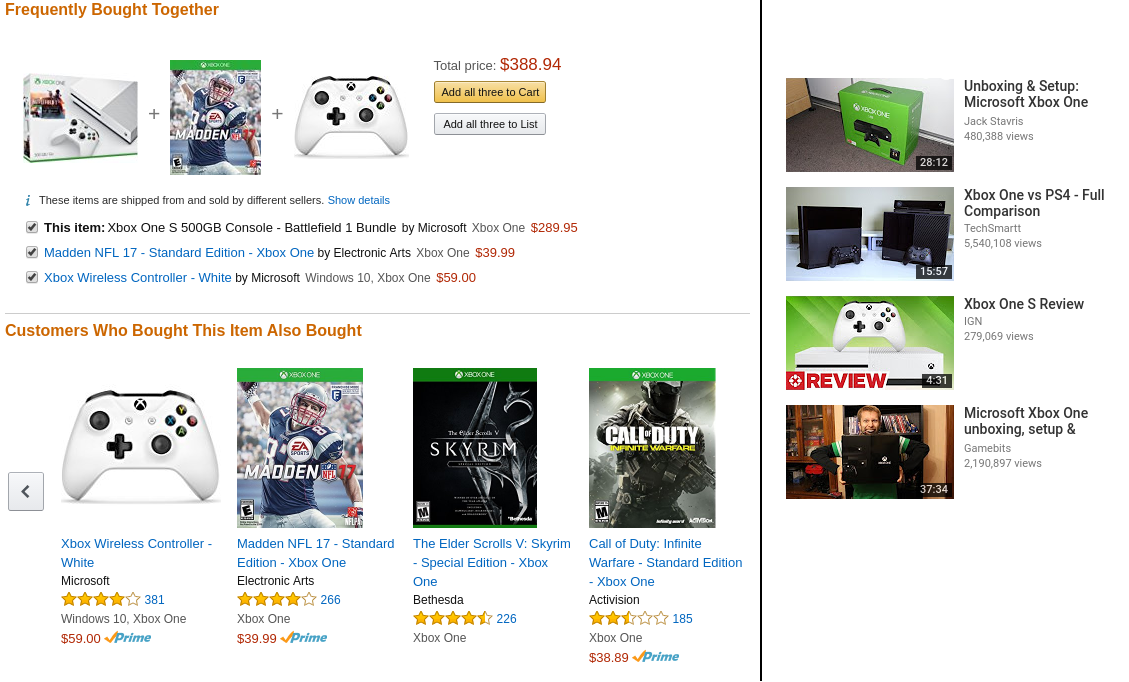
\includegraphics[width=1.1\textwidth]{fig/recsys_example_xbox.png}
	\caption{Recommendations from Amazon (left) and YouTube (right) when looking at Xbox One.}
	\label{fig:recsys-example-xbox}
\end{figure}

Note that there is a subtle difference between predicting which items a user will like, and which items he is interested in interacting with. The former case involves predicting what rating a user will give a movie or whether a user is likely to purchase one or any item. On the other hand, the latter case does not worry about how the user will interact with an item, but whether the user will choose to interact with the item, given the choice. To exemplify this, lets look at a movie streaming site. Should the site recommend movies that the user will rate highly if he watches them, or should it recommend movies that the user is likely to watch independent of how he will rate it? The answer will probably depend on the business and other factors, the point is that there is a difference between the two approaches. In the movie example, it is reasonable to think that how a user would rate a movie is less dynamic than what he want to watch. His ratings would probably depend a lot on his personal preferences, which usually change slowly over time. What he is interested in watching at any point, however, might depend more on circumstances. This was illustrated earlier with the worker who wanted to listen to different genres at during work and his workout session.\\

It is therefore clear that the goal of recommender systems may vary with different businesses and settings. In this paper we are mainly concerned with predicting the next item the user will choose to interact with.\\

There are two classical approaches to recommender systems, collaborative filtering and content-based filtering. These two methods can be combined into a hybrid approach.

\subsection{Collaborative filtering}
Collaborative filtering uses information about users preferences to recommend items highly rated by similar users. To illustrate, let us look at a movie recommendation system. A user logs into a website where he can rate movies he has seen, and the site recommend movies to the user, based on his ratings. With the collaborative filtering approach, the user needs to rate some movies to get good recommendations, and as the user rate more and more movies, the system is able to make better recommendations. To make the recommendations, the system groups together similar users. A user is then recommended movies that he has not seen and that was rated highly by other similar users. The system decides whether users are similar by looking at how like-minded they are, that is, how similar they rate movies. This is illustrated in figure \ref{fig:collaborative-filtering}. The system predicts what rating the question mark will be by guessing the same rating as those given by similar users (highlighted in green).\\

\begin{figure}[htp]
	\centering
	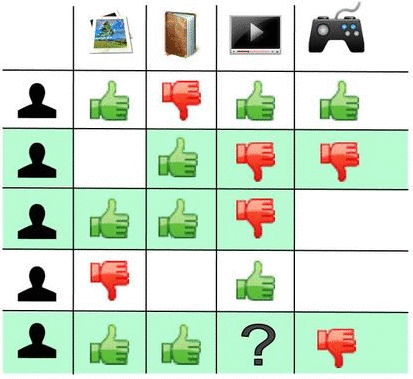
\includegraphics[width=0.4\textwidth]{fig/collab-filtering.png}
	\caption{Illustration of collaborative filtering}
	\source{https://en.wikipedia.org/wiki/Collaborative\_filtering\#/media/File:Collaborative\_filtering.gif}
	\label{fig:collaborative-filtering}
\end{figure}

Many sites have a huge amount of items, and the average user only interacts with a handful of these, this creates a sparsity problem for collaborative filtering methods. These methods also face the cold start problem.\\

One of the most popular collaborative filtering algorithms is matrix factorization \cite{matrix-factorization}.

\subsection{Cold start}
The cold start problem occurs when a recommendation approach is based on having a large amount of data on the user. When a new user occurs the model is not capable of making accurate recommendations due to the lack of user information. Collaborative filtering methods suffers from the cold start problem, but when they do have access to rich user information, they are usually able to make better recommendations than content-based filtering methods.\\

Due to the cold start problem, collaborative filtering approaches alone, are not well suited for session-based recommendations.

\subsection{Content-based filtering}
Content-based approaches builds a user profile based on the item interactions of the user, and features of items. For example, if a user watches a lot of western movies or movies with a certain actor, the system can infer that the user likes the western genre or is a fan of that actor. Then, the system can recommend movies within the western genre or movies where the actor appears. So the approach is to build a user profile based on the profile of the items he interacts with.\\

To achieve good results with content-based filtering, it is important to create accurate item profiles with representative features. The content-based approach does not suffer from the cold start problem to the same degree as collaborative methods, but content-based methods are more limited in their recommendations. They are only able to recommend items similar to those the user has already interacted with. With respect to this, the collaborative filtering approach might offer more valuable recommendations.\\

Some content-based approaches include decision trees, neural networks, and cluster analysis.


\subsection{Session-based recommender systems}
Session-based recommender systems tries to do predictions mostly based on the current user session. Sessions are often limited in time, and, as we have seen, the users interests might vary between sessions. Generally we no information about the user, and since the sessions are short, we do not get much information either. There may be many reasons for this lack of information. Some examples are new users, users sharing accounts, and small e-commerce sites where each unique user only visits it a couple of times. Furthermore, even though we have access to information about the users interest, this might be of minimal use if the users interests vary greatly between sessions. A session usually consists of multiple user actions on a number of items, in the order the actions happen, constrained to a short timespan. What ''short timespan'' means will depend on the domain, but it is often in the order of minutes or a few hours.\\

\subsection{Neural networks}
Neural networks are models inspired by the human brain. They consist of layers of neurons, often referred to as nodes or units, who can receive an input signals, and depending on the strength of the signals, output signals of its own. The nodes are grouped together in layers, and the nodes in each layer output values to the next layer based on the input from the last layer. Values can also be sent back into the same layer they originated from. Each neuron can receive values from multiple neurons, and each neuron can output values to multiple neurons. Each input value to a neuron is weighted, and all the weighted inputs are summed together. A bias might also be added to this sum. This sum is sent through a function, called the activation function, and the function value is passed on to the next neurons. This is illustrated in figure \ref{fig:neural-network}. Mathematically, the layers can be represented as vectors, where each index corresponds to one node, the weights can be stored in a matrix and matrix multiplication can then be used to successively compute the vector for each layer.\\

\begin{figure}[htp]
	\centering
	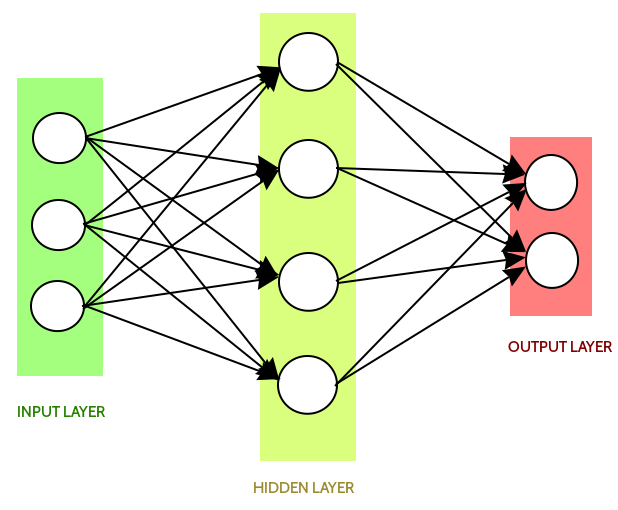
\includegraphics[width=0.8\textwidth]{fig/neural-network.png}
	\caption{A feed forward network. Exmaples are inserted into the network by setting the values in the input layer. The values of the nodes in each layer are computed as a function of the values in the nodes in the prior layer.}
	\label{fig:neural-network}
\end{figure}

An example application might be to let a neural network guess whether it is going to rain in the afternoon, by presenting it with values representing different conditions in the morning. These conditions, or features, could be temperature, air humidity, and whether it rained yesterday. To feed the network these features, they need to be encoded into a vector of real values. This could be done by using a vector with 5 dimensions, where the first index is a 1 or 0, indicating whether it rained or not yesterday. The second index could be the air humidity, scaled down to the range (0,1). And finally, the last 3 indexes could be used to represent the temperature, for example, by creating three buckets. If the temperature is above 20 \degree C, the third index would be set to 1, the fourth if the temperature is between 0 \degree C and 20 \degree C, and the fifth index would be used if the temperature is below 0 \degree C. The output layer could be a vector with 2 dimensions, where one index would indicate rain, and the other would indicate no rain. Then the index with the highest value could be used as the networks prediction.\\

The layers between the input and the output layers are called hidden layers. A neural network can any number of hidden layers, this includes not having a hidden layer at all. The width of a layer is the number of nodes in the layer. Adding more layers to a network increases its capacity, which means that it becomes capable of solving more complex problems. However, with more layers, the network also becomes harder to train, both in terms of number of calculations and because more layers creates a bigger, and more complex search space.\\

The most popular ways of training uses backpropagation. Different variations exists, but the main idea is the following. First the network is presented with an example, and the values of all the nodes in the network is computed. Error values are calculated for the output layer, based on its difference from the target output. These errors are then backpropagated through the network. This means that the error in each node is dependent on the input it gets from the previous, upstream, nodes. So the error of the upstream nodes can be calculated by how much they contributed to the error in the downstream nodes. Based on this, the weights in the network can be adjusted. Let us look at a very basic example. A single output node, \textit{O}, ends up with the value 1. This is the sum of 2 and -1, which \textit{O} got from nodes \textit{A} and \textit{B} respectively. If the target value of \textit{O} was 0.5, then the weights from \textit{A} and \textit{B} to \textit{O}, should be adjusted so that the sum of the inputs gets skewed towards 0.5. So after the adjustments, \textit{A} and \textit{B} would output 1.75 and -1.25 instead, on the same example. Exactly how the weights are updated, depends on the chosen training algorithm and the parameters used, but the main idea is mostly the same.\\

In more correct terms, the output error is calculated with a loss function. Greater error means greater loss. But the loss does not have to be as simple as the difference between the target values and the computed values, more delicate functions can be applied. The most successful algorithm for training neural networks is called backpropagation and was introduced by Rumelhart et al. in 1985 \cite{DBLP:journals/corr/Lipton15} \cite{Rumelhart:1986:LIR:104279.104293}. Backpropagation uses the chain rule to calculate the derivative of the loss function L with respect to each parameter in the network. The weights are then adjusted by gradient descent \cite{DBLP:journals/corr/Lipton15}.

Figure \ref{fig:neural-network} shows a fully connected feed forward network. Fully connected means that each node in a layer is connected to all the nodes in the next layer. Feed forward means that there are no cycles or recurrent connections, all connections go to the next layer, towards the output layer.

\subsection{Dropout}
Dropout is a regularization technique that can be used when training neural networks. As the name implies, a subset of the nodes are deactivated. Deactivating subsets of the nodes during training, can help avoid overfitting and it can speed up the training \cite{Srivastava:2014:DSW:2627435.2670313}. Speed up is achieved because there are less nodes to train. By randomly deactivating node, the network becomes more robust, since it cannot rely to much on any one node to produce good results.

\subsection{Minibatches}
When training neural networks, one can calculate the error for multiple training examples and then update the weights based on the average of these examples. These groups of examples are called minibatches. There are several benefits of using this. Using large batches generally results in a more accurate estimate of the actual error of the model. For example if some of the examples are outliers. With a better estimate of the real error, the training algorithm can use a higher learning rate. Also, some hardware can be better utilized when training with batches. \cite{Goodfellow-et-al-2016-Book}

\subsection{Deep learning}
The small network shown in figure \ref{fig:neural-network} is not capable of learning very complex tasks, it is too simple.  Increasing the size of the layers would probably give it some more capacity. If we wanted to do image labeling, the task of recognizing objects in an image, with it we could increase the input layer so that it had three nodes for each pixel (RGB). We would also have to increase the output layer to have one node for each possible label. However, even with a huge hidden layer, the model will struggle to make sense of raw pixels with only a few calculations. To help the model, we could give it additional input, we could tell it whether geometric figures like circles exists in the image. But by doing this, we have started to do some of the image labeling ourselves. Also, the model is dependent on us being able to find good features for it. We want the model to do most of the work for us. It would be nice if the model could extract good features by itself. It turns out that it can.\\

By adding more hidden layers to our model it becomes much more capable. In its simplest explanation deep learning is just that, using more layers. This does not just apply to neural networks, one can also stack layers of other artificial intelligence methods, but we will focus on neural networks. The great benefit of using deep models is that the models are able to learn and extract good features themselves \cite{Goodfellow-et-al-2016-Book}. In the case of image labeling, the first layers can learn to extract features like edges and simple shapes. The deeper layers can then use these features to recognize more complex shapes in the image. Or in the case of recommender systems, the model can learn to extract features from the items and user preferences from user actions. Deep learning lets the machine learn hierarchical concepts, giving it more power and flexibility \cite{Goodfellow-et-al-2016-Book}.

\subsection{Recurrent neural networks}
Recurrent neural networks(RNN) area form of neural network that is suited for processing sequences of data. Standard neural networks have no form of memory between examples, they assume that each example is independent, which often is not true. RNN solve this by using loops where information from the one time step is passed on to the next one. This gives the model memory, and it does not need to assume independence between examples. It also means that the model is more suited for sequences of varying lengths. Figure \ref{fig:rnn} illustrates a basic RNN. It can be illustrated both as a loop and as an unrolled network. Note that, as implied by the looped representation, the RNN is the same across all time steps. In the unrolled version, the RNN boxes are the same network, there are not \textit{t} different RNNs that are connected.\\

\begin{figure}[htp]
	\centering
	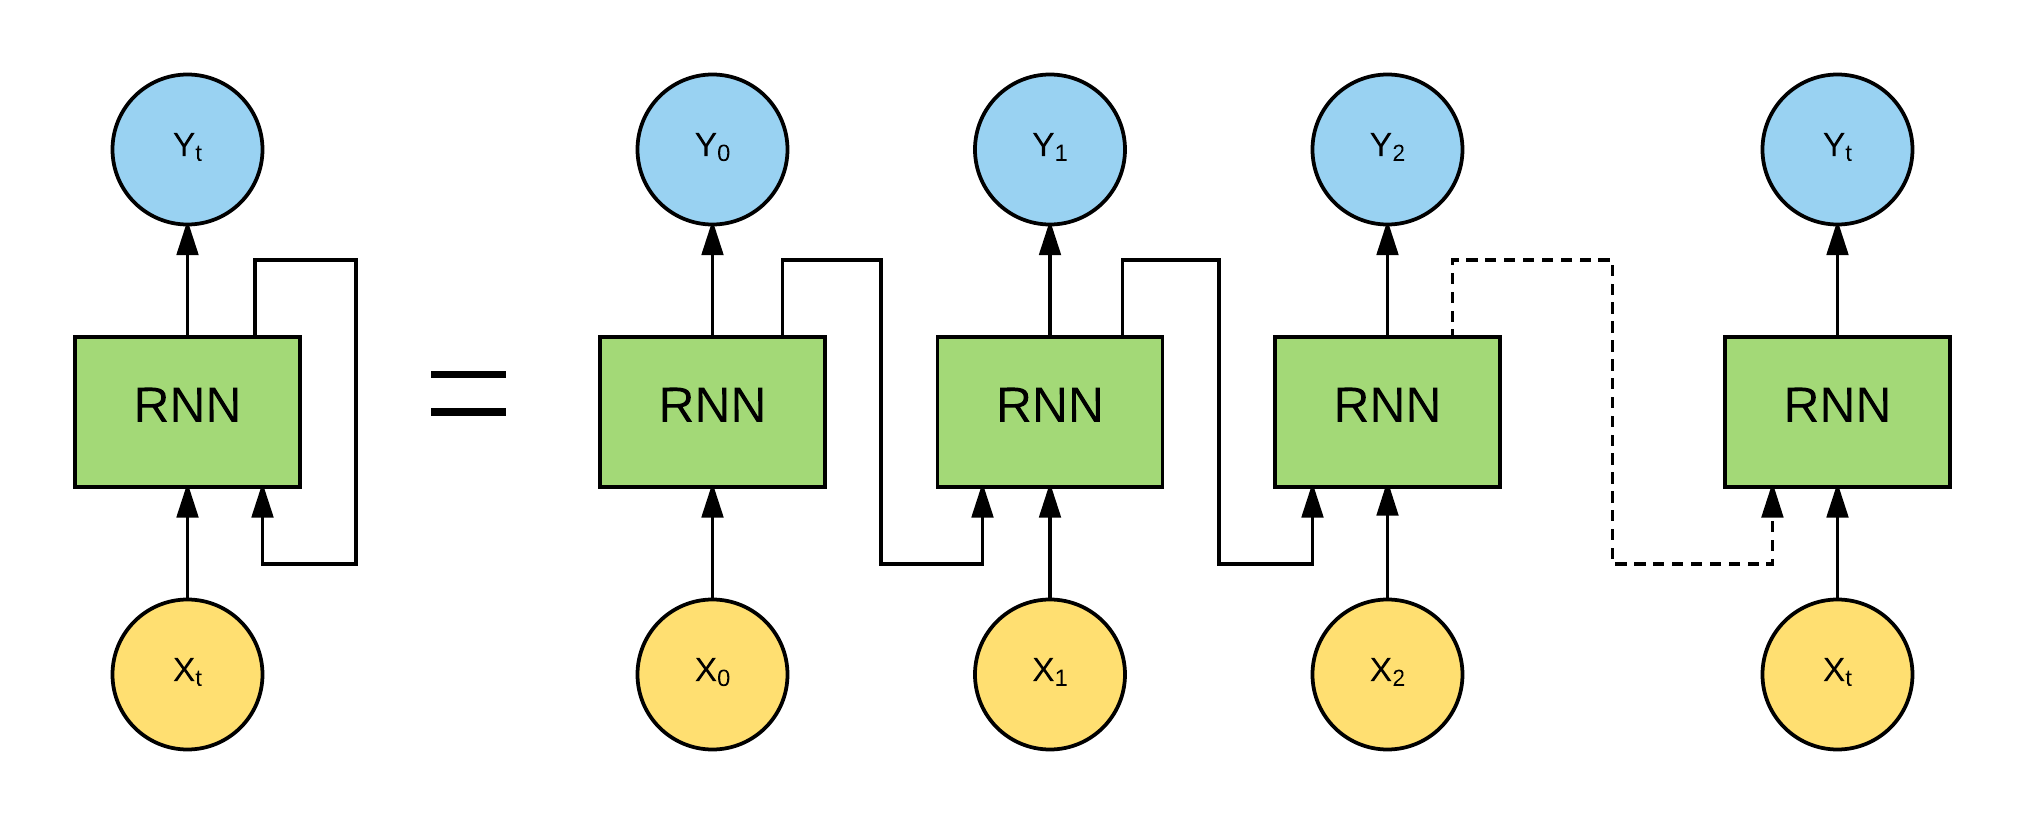
\includegraphics[width=1.0\textwidth]{fig/rnn.png}
	\caption{A simple RNN. Represented as a loop(left), and unrolled to \textit{t} timesteps(right).}
	\label{fig:rnn}
\end{figure}

At each time step, the network takes in external input and input from the last time step, two outputs are created. One output is passed on to the output layer, or the next hidden layer if there is one. The other output is the state of the RNN, which is passed on to the next time step. Each time step does not have to be separated by a fixed amount of time, each time step is just when input arrives. It is fully possible to apply deep learning to RNNs. One can stack multiple RNNs, or add other types of layers such as a plain feed forward layer.\\

RNNs are not constrained to neither fixed sized inputs nor outputs. The size of input and output \textit{vectors} are fixed, but RNNs are not limited to a fixed number of such vectors. However, RNNs can be applied both to domains where it is natural to treat the data as sequences, as well as problems where the amount of input is fixed. An example of this is to use a RNN as a sliding window over fixed sized images.


\subsection{LSTM and GRU}
Early RNN had troubles with training because of vanishing and exploding gradients. When using many time steps the gradients often grew too steep, exploded, or they approached zero, vanished. This problem happened because the recurrent edge in a node always had the same weight, which resulted in the derivative of the error either exploding or approaching zero, at an exponential rate, as the number of time steps grew \cite{DBLP:journals/corr/Lipton15}. This was solved by introducing a memory cell. The new model introduced by Hochreiter and Schmidhuber in 1997 and is called \textit{long short-term memory}(LSTM) \cite{Hochreiter96bridginglong}. Improvements to the original model has been made over time. In the LSTM model, each node in the recurrent layer is replaced by a memory cell. The internal structure of the memory cell is a bit complex, but simply explained it has an internal state that it can modify, in addition to the old features of RNN nodes. So, the cells can decide how much information in the internal state they want to keep at each time step, and how much new information they want to add.\\

GRU

\subsection{RNN as a session-based recommender system}
Explain how RNNs fit into the session-based context

%theoretical background. explain everything at a high level (more technical explanations can be done in state of the art). Everything that is used in the core

%- What is a recommender system?
%   Why do recommender systems exist
%   Two sligthly different types of recommender systems (predict what the user will give a good rating, and predict what the user would want to interact with independently of whether he will give it a good rating or not)
%- What is a session-based recommender system?
%- What is a neural network
%- What is deep learning
%- What is RNN
%- GRU and LSTM
%- Contextualise what I am doing
%- what is contextual information (external [time, weather, ...] and item specific context [more info abiout the item: image, text, category...])

%-----------------------
%- explain the problem domain
%- explain rnn
\chapter{State of the Art}
\label{chp:sota}
In this chapter, we examine work that has been done on the use of deep learning for recommender systems. We are interested in the use of RNNs and the session-based recommender system setting.

\section{Other approaches}
Here we briefly mention some of the most used or successful non-RNN approaches to recommender systems.

\subsection{The item-to-item approach}
In recommender systems where a user profile is available, Matrix factorization and neighborhood models have been among the most popular approaches. Due to the missing user information in the session-based scenario, these methods do not work well there. In session-based recommendations, a popular approach is item-to-item recommendation. The item-to-item method precomputes a similarity matrix for the items. Items who are similar, based on the available session data, get high scores, and recommendation is done simply by recommending similar items. Similarity is calculated by looking at which items are often clicked in the same sessions. This method is simple and effective, and has been widely used \cite{DBLP:journals/corr/HidasiKBT15}. However, it only considers the last click.

\subsection{Markov models}
Markov models can representing time dependencies. Hidden Markov models model an observed sequence as probabilistic dependent on a sequence of unobserved states \cite{DBLP:journals/corr/Lipton15}. The problem is that as the time window grows, the state space grows exponentially. This makes Markov models infeasible on longer sequences. RNNs do not have this problem, because the number of states that can be represented grows exponentially with the number of nodes in a layer. In addition, the complexity of inference and training grows at most quadratically \cite{DBLP:journals/corr/Lipton15}.

\subsection{Deep learning}
Restricted Boltzmann Machines (RBM) have successfully been used for collaborative filtering \cite{Salakhutdinov:2007:RBM:1273496.1273596} \cite{DBLP:journals/corr/HidasiKBT15}, and has been shown to be one of the best performing models for that approach. The RBM model performs recommendations by modeling user-item interactions.

Deep models have been used to extract content features, and then combined with a collaborative filtering model to enhance the results \cite{DBLP:journals/corr/WangWY14} \cite{Oord:2013:DCM:2999792.2999907} \cite{DBLP:journals/corr/HidasiKBT15}.

In 2015, Wan et al. \cite{conf/recsys/WanLWGXC15} experimented with a three-layered neural network for next basket recommendation. A basket here refers to the shopping basket on an e-commerce site. So, the setting is an e-commerce site where users have done some purchases, and where each purchase consists of a basket with one or more items. In this scenario, the recommender system has access to the user's history, so it is not a session-based problem. Wan et al. argues that recommendations should be based on the full user history, not only the last purchases. To illustrate, a user might purchase a computer, then he might purchase groceries in his next basket, and then he wants to buy some accessories to his computer. They feed the network with the user history by creating vectors that represent the average of each basket, and creating an embedded concatenation of these vectors. Their network outperforms the baselines they compare it to.

\begin{figure}[htp]
	\centering
	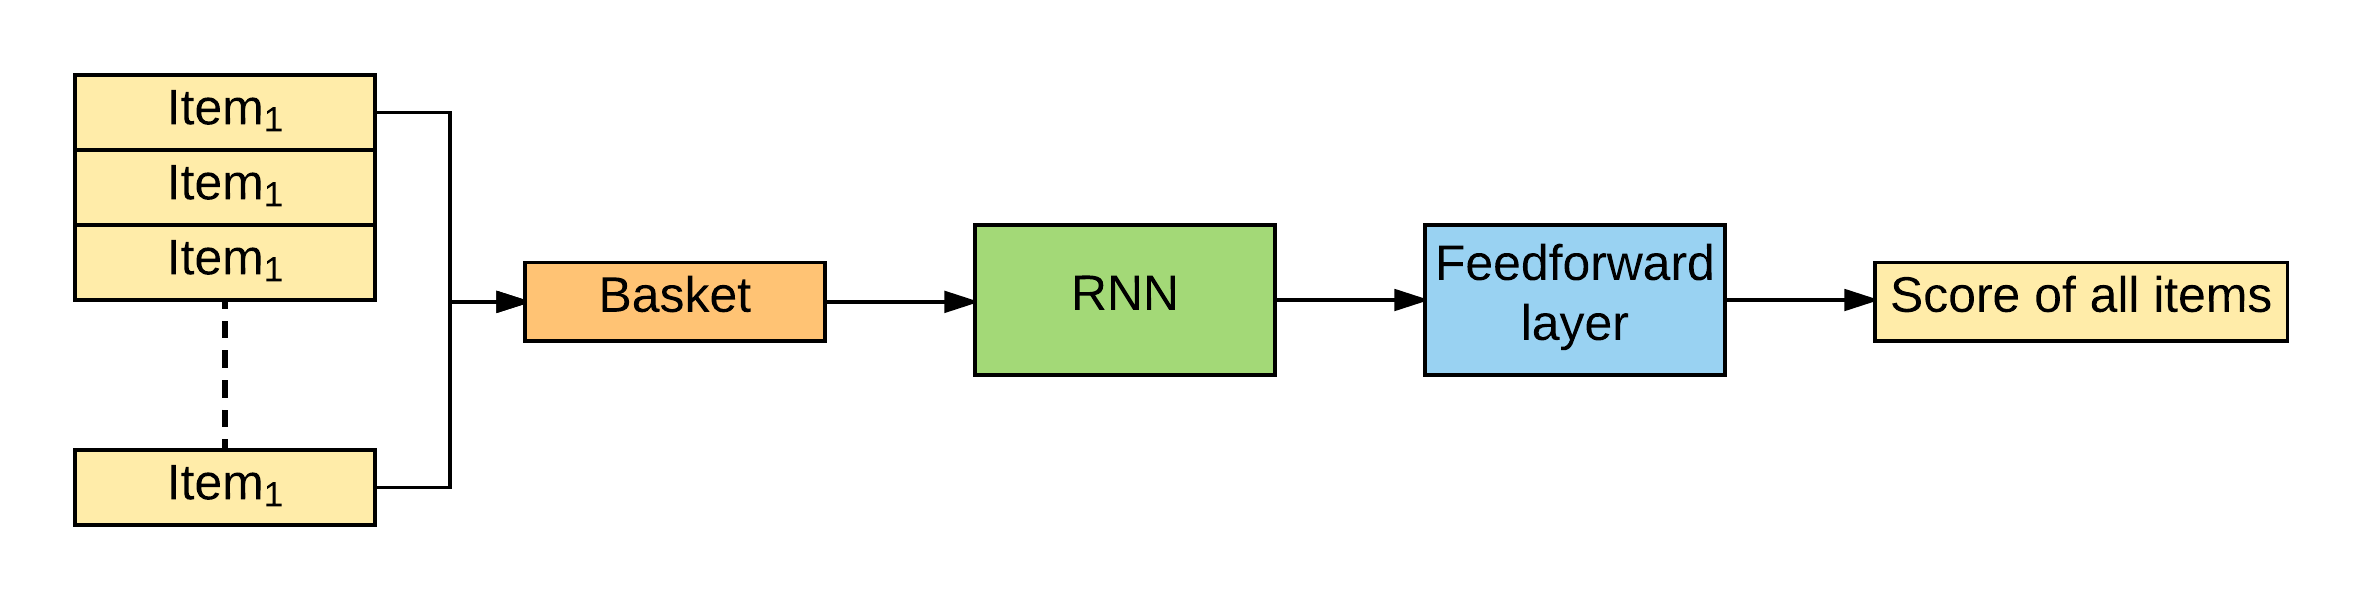
\includegraphics[width=1.0\textwidth]{fig/rnn-next-basket.png}
	\caption{General architecture of the RNN from ''A dynamic recurrent model for next basket recommendation'' by Yu et al. \cite{Yu:2016:DRM:2911451.2914683}}
	\label{fig:rnn-next-basket}
\end{figure}

A paper by Yu et al. from 2016 \cite{Yu:2016:DRM:2911451.2914683} suggests using a RNN to perform next basket recommendation. Their network architecture is illustrated in Figure \ref{fig:rnn-next-basket}. They represent each user basket by pooling together the item vectors in the basket. The basket representation is sent through a simple RNN and outputs a vector with a score for each item. Their model performs better than the baselines over two datasets. This is not a session-based recommender system, but in the next section we look at a paper that applies a similar model as a session-based recommender.


\section{Session-based recommendations with recurrent neural networks}
\label{sec:hidasi-sess-based-rnn}
Hidasi et al. published the paper ''Session-based Recommendations with Recurrent Neural Networks'' in 2016 \cite{DBLP:journals/corr/HidasiKBT15}. This paper proposes to use a RNN for session-based recommendations, and shows that a basic RNN can achieve remarkable results. They also deal with sparsity issues, and introduce a new ranking loss function for training the network. Their general network architecture is shown in Figure \ref{fig:gru4rec-network}. We discuss their network in detail in the next subsections.

\begin{figure}[htp]
	\centering
	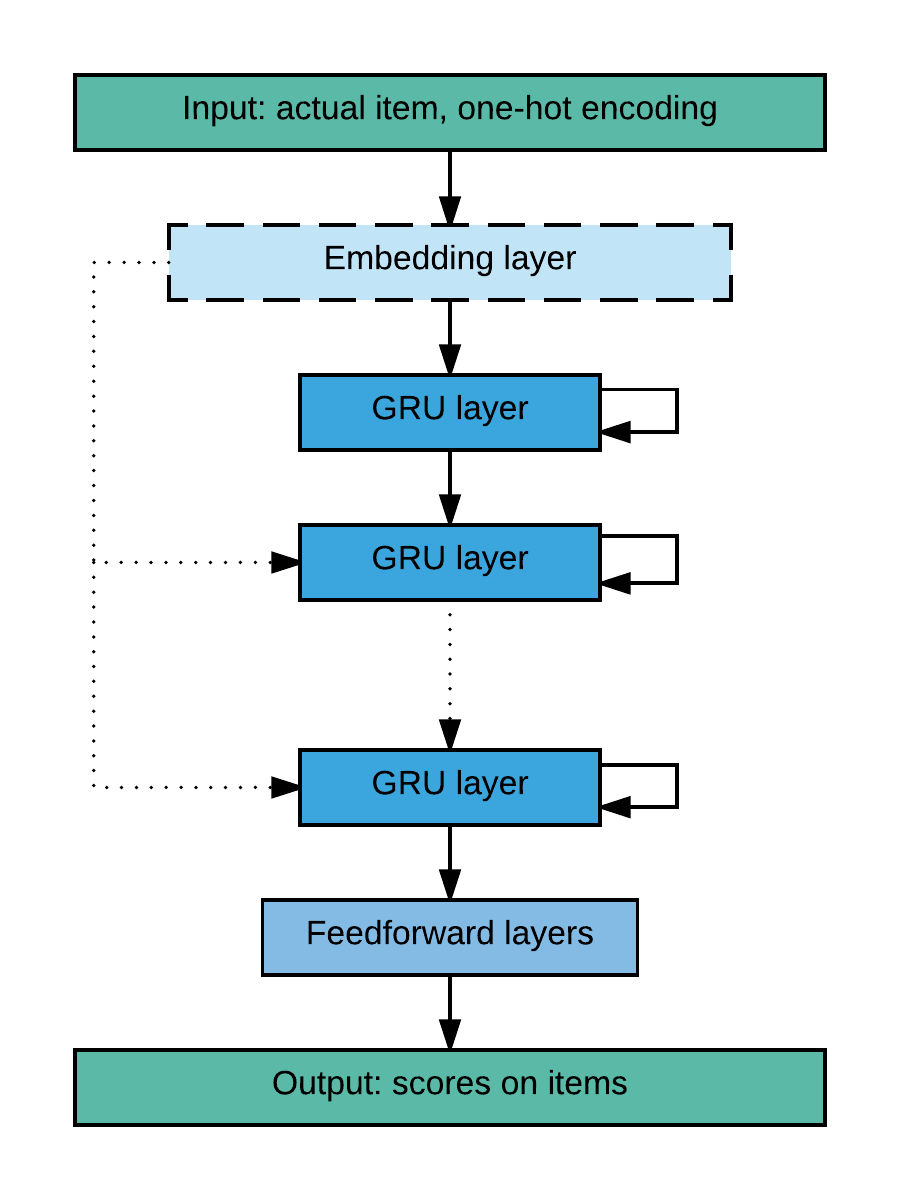
\includegraphics[width=0.5\textwidth]{fig/gru4rec-network.png}
	\caption{General architecture of the RNN from ''Session-based recommendations with recurrent neural networks''. \cite{DBLP:journals/corr/HidasiKBT15}}
	\label{fig:gru4rec-network}
\end{figure}

They experimented with two different datasets. Both datasets contain sequences of user clicks with timestamps. One dataset has clicks on items from an e-commerce site from the RecSys Challenge 2015 \cite{dataset:recsys15}, while the other contains clicks on videos from a YouTube-like platform. Various modifications of the network in Figure \ref{fig:gru4rec-network} were tested. We discuss these as we explain the architecture, layer by layer.

\subsection{Input layer}
Two different ways of encoding the input were compared. The first encoding was a pure one-hot encoding. The second was a weighted sum of the first representations, where earlier events are discounted, and the entire vector was normalized before fed into the network. Adding information about all earlier events could possibly help to reinforce the memory effect. However, in this case the RNN performed better with the pure one-hot encoding. 

\subsection{Embedding layer}
In the paper, the authors mention that they experimented with using an embedding layer between the input- and the RNN layer. Their results were always better without the embedding layer. However, if the performance loss is small, an embedding layer can still be useful to speed up calculations, as mentioned in \ref{sec:embeddings}. In the recommender system setting, the number of possible items can be very large, also the system need to be responsive, so potential speed optimizations should be considered.

\subsection{GRU layers}
GRU units outputs a hidden state and an output which is the prediction for the time step. The hidden state from each layer is inputted back into the same layer for each time step, but it is also fully possible to output the hidden state to the next layer, instead of or in addition to the prediction output. The authors experimented with using multiple GRU layers, where they used the hidden state as output to the next layer, except for the last GRU layer which outputted the prediction output. Best performance was achieved with a single GRU layer. It is not clear why additional layers did not improve the result, but as the authors mention, it might be because the sessions have short lifespans. If the sessions spanned over weeks, then additional layers could catch user features at different time scales. I.e. one layer could learn the more static features of the user, features which does not change over the whole session, while another layer could learn the more temporal user features, features that were only present for the past hour for example. It was also found that, when using multiple GRU layers, feeding the input, the one-hot- or the embedded vector, into the deeper GRU layers resulted in better performance.

\subsection{Feedforward layers}
In the paper, they found that using a single feedforward layer gave the best results. The feedforward layer maps a smaller vector to the same size as the input layer, where each item corresponds to one index again. By having a feedforward layer between the GRU layer and the output, the GRU layer can be much smaller. Since a GRU layer is more complex than a feedforward layer, it is also slower in terms of computations. In recommender systems, the number of items can span from thousands to millions. Therefore, keeping the GRU layer small can be necessary to achieve a feasible runtime.

\subsection{Training}
The e-commerce dataset has about 40 000 items, while the video dataset has about 330 000 videos. Therefore, the paper samples the output, and only calculates scores for some of the outputs. The network outputs a score for each item, since the output vector contains one value in each index. The correct output is one where the desired item, the next one in the session, has a higher score than the others. There are at least two reasons why the other items in each time step were not clicked. One possibility is that the user did not see the item, another possibility is that the user saw the item, but chose to not click it because it was not interesting to him. For popular items, the second reason is more likely, and it is important that the network learns to give these items a low score. In the paper, this is solved by using the items from the other examples in the current mini-batch as negative examples, and of course, the next click is the positive example. By using clicks from the other examples in the mini-batch, computations for sampling is saved, in addition, these clicks are automatically sampled by proportion to how popular they are, because popularity is decided by number of clicks.

In the paper, Bayesian Personalized Ranking \cite{Rendle:2009:BBP:1795114.1795167}, TOP1 (devised by the authors \cite{DBLP:journals/corr/HidasiKBT15}), and cross-entropy are used to calculate the loss. With 100 units in the GRU layer, cross-entropy performed best. With 1000 units, TOP1 performed best overall, but was beaten by BPR on one metric. TOP1 performed better with 1000 units than cross-entropy did with 100.

\subsection{Evaluation metrics}
\label{sec:evaluation-metrics}
The paper suggests two performance metrics suited for recommender systems.

\subsubsection{Recall@N}
In cases where the recommender system can recommend a set of N items, and the full set is visible to the user, it is important that good recommendations are in the set, but the ordering does not matter. The Recall@N measure is then how often the correct next click is present in the top N recommendations by the recommender system. The top N recommendations are the N items with the highest score given by the system.

\subsubsection{MRR@N}
When the user needs to do some form of scrolling to see all recommendations, the order of the recommendations becomes important. The best recommendations should be the first visible to the user. Mean reciprocal rank (MRR) covers this case. MRR@N measures the average of the reciprocal rank of the correct click in the systems N recommendations. The recommendations need to be ordered by the recommender. If the system recommends 20 items, then it gets a score of 0 if the correct prediction is not in the list of recommendations. If the correct prediction is in the list, the system gets a score of $\frac{1}{i}$, where $i$ is the rank in the list. So if the correct item is first in the list, the score is $\frac{1}{1} = 1$, and if it is number five in the list, the score is $\frac{1}{5} = 0.2$. The MRR@N is the average of these scores over all the test examples.

\subsection{Results and conclusion}
The RNN in the paper was compared to several baselines. The best performing baseline was the item-KNN. Item-KNN recommends items based on similarity, where the similarity is calculated based on items co-occurrences in sessions. This similarity is calculated with the cosine similarity between the vector of the sessions where both items occur. Specifically it is ''the number of co-occurrences of two items in sessions, divided by the square root of the product of the number of sessions in which the individual items occurred'' \cite{DBLP:journals/corr/HidasiKBT15}.

This simple item-to-item method is usually a strong baseline, and often used in practice. The paper's proposed RNN significantly outperforms the item-KNN baseline with about 15 - 30 \% higher accuracy scores on the two evaluation metrics. The paper by Hidasi et al. has given us a solid RNN, with a relatively simple architecture. It performs well even though it only looks at the sequences of item clicks. No additional information about the items are fed into the network. The next papers we discuss looks at methods that can be used to further improve results.



\section{Improving RNNs for session-based recommendations}
\label{sec:improved-rnn}
Tan et al. \cite{DBLP:journals/corr/TanXL16} looks at various ways of improving the model proposed by Hidasi et al. in \cite{DBLP:journals/corr/HidasiKBT15}. They experiment with techniques that have worked well when neural networks have been applied to other problems, to see if those techniques can improve performance of a RNN session-based recommender as well. The same evaluation metrics, Recall@20 and MRR@20, were used, and they experimented on the same dataset from RecSys CHallange 2015 \cite{dataset:recsys15}. They suggest four techniques, and train one model with each technique. The four models are then compared with each other and a baseline which is the model proposed by Hidasi et al. in \cite{DBLP:journals/corr/HidasiKBT15}.

\subsection{Data augmentation}
Based on \cite{DBLP:journals/corr/BrebissonSAVB15}, they generate multiple sequences from each sequence in the original dataset. For a sequence \lbrack $x_1$, $x_2$, ..., $x_n$\rbrack, they create sequences \lbrack $x_1$, $x_2$\rbrack, \lbrack $x_1$, $x_2$, $x_3$\rbrack, ..., \lbrack $x_1$, $x_2$, ..., $x_{n-1}$\rbrack, in addition to the original sequence. The last click in each sequence is used as the target click.

Another form of data augmentation they suggest is dropout performed on the clicks in the training sequences. This is based on results from \cite{rnn-dropout}. By randomly dropping clicks in the training sequences, the model could become less sensitive to noise clicks, which makes the model less prone to overfitting on noise. Both methods are illustrated in Figure \ref{fig:sequence-augmentation}. The model described in this section will be referred to as M1.

\begin{figure}[htp]
	\centering
	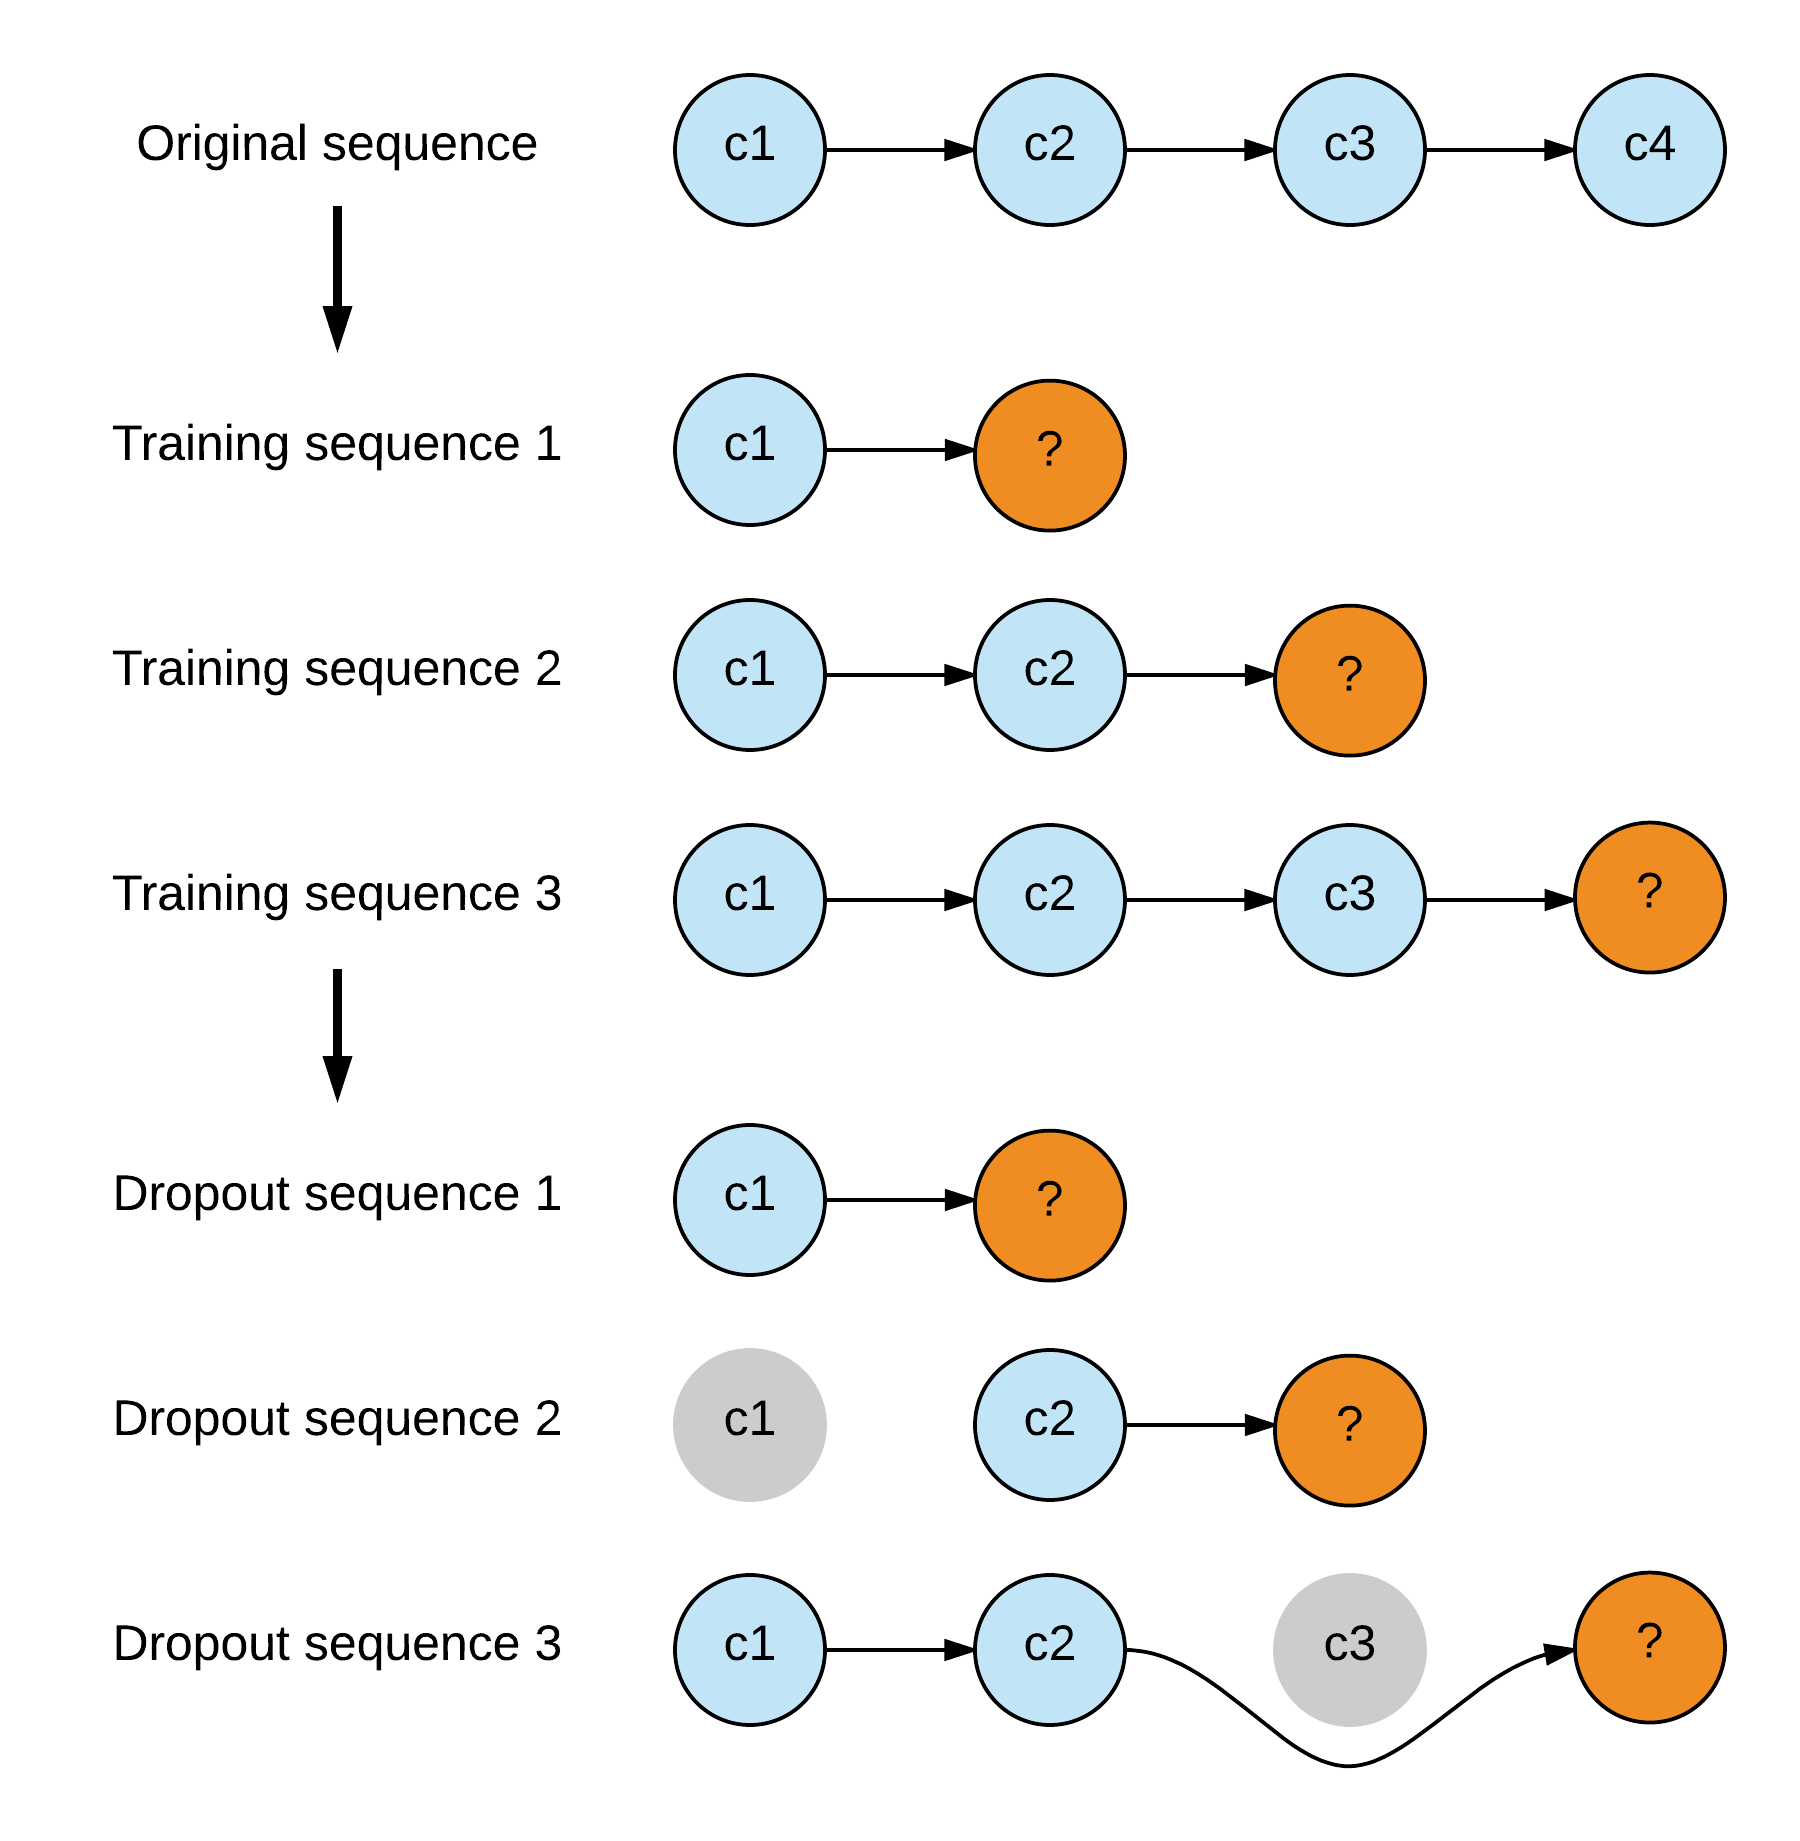
\includegraphics[width=0.7\textwidth]{fig/sequence-augmentation.png}
	\caption{Data augmentation for training sequences as suggested in \cite{DBLP:journals/corr/TanXL16}. Multiple training sequences are generated from the original sequence. Random dropout is applied to the clicks in the sequences.}
	\label{fig:sequence-augmentation}
\end{figure}

\subsection{Pre-training to adapt to temporal changes}
In the session-based setting, the items available for recommendation changes over time. One of the consequences is that users interest change over time, as newer items are often more exciting than old ones. These changes will be reflected in the training sequences, where the most recent examples more correctly reflect users' current interests. Naturally, the recommender system should be in sync with the users' current preferences. One obvious solution is to discard examples from the dataset that are older than a certain threshold. However, this means a lot of data is lost. It would be better if this data could be utilized. Tan et al. suggests that a good solution is to apply pre-training. First the model is trained on the whole dataset, then it is fine-tuned on only the most recent examples. This results in a model that makes use of the full dataset, but which is focused more on the recent tendencies. This idea is based on the fine-tuning often used on image-based networks \cite{DBLP:journals/corr/ChatfieldSVZ14}. The model described in this section will be referred to as M2.

\subsection{Privileged information}
When training on a subsequence of a session, there is still the remaining part of the sequence which contains information about the session. Tan et al. proposes to use this information as well when training. Look at Figure \ref{fig:rnn-teacher-student} for an illustration.

\begin{figure}[htp]
	\centering
	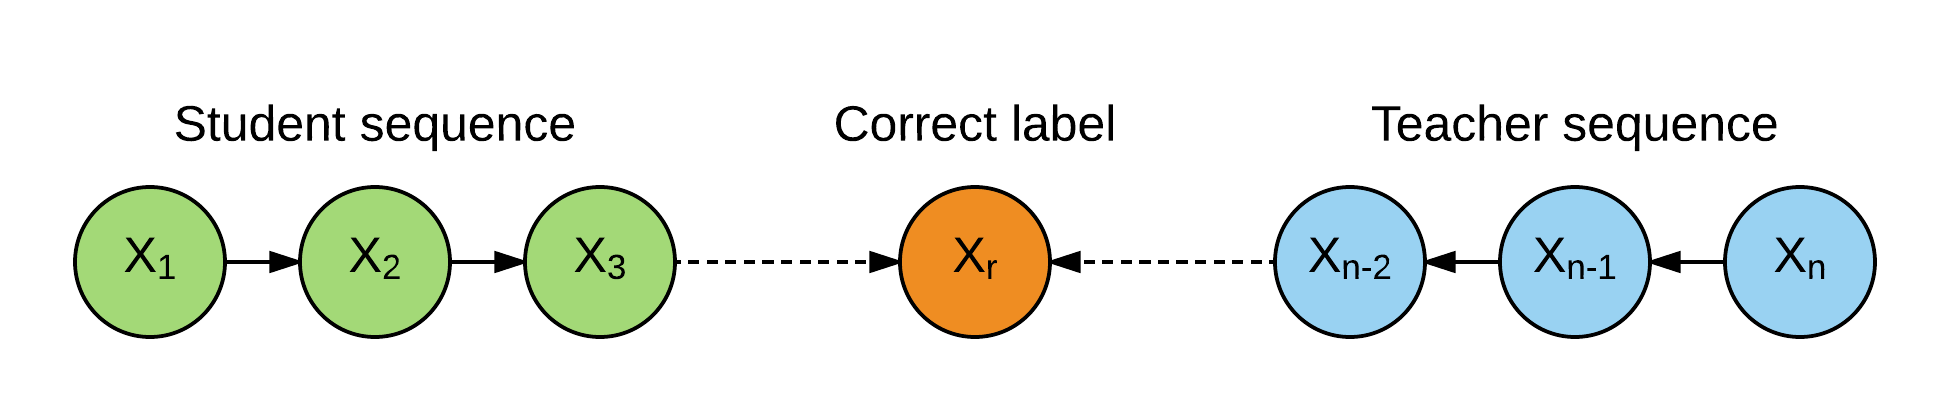
\includegraphics[width=1.0\textwidth]{fig/rnn-teacher-student.png}
	\caption{Data augmentation with teacher labels as suggested in \cite{DBLP:journals/corr/TanXL16}. The student model is trained to predict a tradeoff between the real label and the label predicted by the teacher model. The label produced by the teacher model is the teacher model's prediction of the correct label but on the remainder of the sequence in reverse.}
	\label{fig:rnn-teacher-student}
\end{figure}

For some sequence \lbrack $x_1$, $x_2$, ..., $x_r$, ..., $x_{n-2}$, $x_{n-1}$, $x_n$\rbrack, where $x_r$ is the label, the model is being trained to predict $x_r$ based on \lbrack $x_1$, $x_2$, ..., $x_{r-1}$\rbrack. This is normal training as we have already looked at. The addition is that the label that the model is trained to predict is substituted with a tradeoff between the correct label and a label produced by a teacher model. The label produced by the teacher model, is the teacher model's prediction of the correct label, $x_r$ based on the reverse of the remaining sequence, which is \lbrack $x_n$, $x_{n-1}$, ..., $x_{r+1}$\rbrack. This approach can be useful when the available training data is small, such as for new websites \cite{DBLP:journals/corr/TanXL16}. The model described in this section will be referred to as M3.

\subsection{Output embeddings}
The number of possible items to recommend can be huge. Therefore, outputting a vector of size equal to the number of items will requires a lot of calculations, which means that the model can become less responsive (slow to calculate an output). To deal with this \cite{DBLP:journals/corr/TanXL16} suggests to output an item embedding instead of a full item vector. Since the embedding is a smaller vector, this means less calculations and faster predictions. The top N recommendations are extracted from the output embedding by finding the item's most similar embeddings in the embedding space, where similarity is calculated with cosine similarity. For this to work, the model needs to have good embeddings to train on. The authors suggest using the embeddings found with one of the other models for this. The model described in this section will be referred to as M4.

\subsection{Results and conclusion}
The RecSys Challange 2015 dataset was preprocessed and split into test and training sets in the same way done by Hidasi et al. in \cite{DBLP:journals/corr/HidasiKBT15}. To better evaluate their models, the authors sorted the examples in the training set by time, and compared the models using the most recent fractions ($\frac{1}{256}$, $\frac{1}{64}$, $\frac{1}{4}$, $\frac{1}{1}$) of the training sequences. The same evaluation metrics were used. As baseline, the pest reported results from \cite{DBLP:journals/corr/HidasiKBT15} were used. The results are shown in Figure \ref{fig:improved-rnn-results}

\begin{figure}[htp]
	\centering
	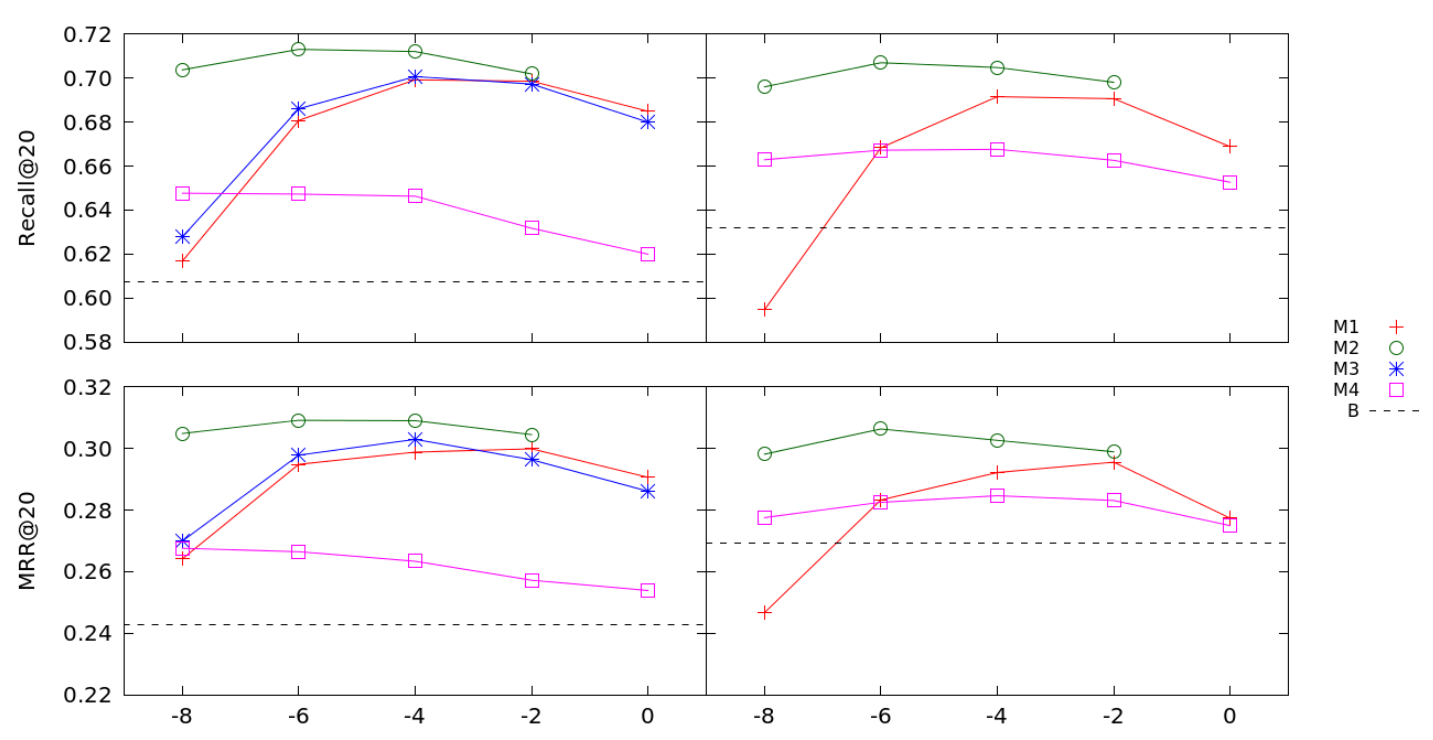
\includegraphics[width=1.0\textwidth]{fig/improved-rnn-results.png}
	\caption{Results from \cite{DBLP:journals/corr/TanXL16}. \textbf{B} is the baseline, which is the reported performance from \cite{DBLP:journals/corr/HidasiKBT15}. ''Plots of both evaluation metrics on models with GRU size 100 (left) and 1000 (right). The x-axis is logarithmic in dataset fraction, the rightmost point corresponds to the full dataset. M2 does not apply to the full dataset, and results for M3 on the larger GRU size were omitted'' \cite{DBLP:journals/corr/TanXL16}}
	\source{''Improved recurrent neural networks for session-based recommendations'' by Tan et al. \cite{DBLP:journals/corr/TanXL16}}
	\label{fig:improved-rnn-results}
\end{figure}


Except when only using the most recent fraction of the training data ($\frac{1}{256}$), all proposed models, M1-M4, performed better than the baseline. M4 generally performed worst of the four models. M2 performed best, especially on the most recent fractions. M2 was not trained on the whole training set, since that would be equivalent to recreating the baseline. M1 and M3 performed best when trained on $\frac{1}{4}$ and $\frac{1}{16}$ of the most recent training examples. At best, M2 achieved about 10 percentage points better on Recall@20 and about 8 percentage points better on MRR@20 than the baseline. However, it might have been a bit unfair to use the reported performance from \cite{DBLP:journals/corr/HidasiKBT15} as a baseline. Hidasi et al. did many optimizations to make their model run faster \cite{email:Hidasi}, and some of the tricks they used might have lowered the models performance (in terms of Recall@20 and MRR@20) in a tradeoff for faster runtime. The M2 model trained on the full training set would probably have been a fairer baseline to compare the models to. Based on the results for M2 on the fractions of the training set it was trained on, it seems reasonable to believe that M2 would have gotten a significant better score than the baseline when trained on the full training set.

Still the paper presents some nice ideas on how to improve a RNN session-based recommender. Dropping some of the oldest data can improve the results for any model. Also, the M4 model had about half the prediction time of the other models, which is useful in cases where one wants to do a tradeoff.


\section{Utilizing context information}
So far, we have looked at models that performs predictions solely based on the items clicked, where the items are only represented by an ID in the form of a one-hot vector. Clearly, additional information, both about the item and about the sessions, could help improve the predictions. Some possible additional information about the item is be the category of the item, an image, and a textual description of the item. Additional information about the session could be timestamps of the clicks, geolocation of the user, and weather. In this and the next sections, we discuss papers that examine if and how additional information can improve a RNN recommender.

We start in this section by looking at ''Context-aware sequential recommendation'' by Liu et al. \cite{DBLP:journals/corr/LiuWWL016}.

The paper suggests that modeling the time of a session and the transition time between events in the session both can give better performance. Modeling time, such as hour of the day and day of the week, can help the model capture tendencies that depend on when a session occurs. As an example, think of a music streaming service. During working hours on the weekdays, users might listen more to calm music which helps them concentrating. On the evening in the weekend, there might be a rush in users listening to party music at parties. And music preferences might vary with the seasons of the year. The authors refer to this as input contexts.

Time between actions in a session might give an indication about how relevant actions are to each other. Intuitively, actions that happens in short time intervals should be more relevant to each other, and vice versa. This could help the RNN decide when to what and when to forget and remember. The authors refer to this as transitional contexts.

Liu et al. proposes to define a finite number of input and transitional contexts and then give the recommender model one layer for each context. When an example is given to the model, it uses only the appropriate layers, and similarly training is done on the layers that were used for the example. More technically, the item input vector is multiplied with an input context matrix, and the hidden state vector is multiplied with a transition context matrix, in each step in a sequence. It is these matrices that the authors suggest to generate for each possible context. The input contexts used in the paper are 24 hours of the day, seven days of the week, three ten-day periods in a month, and holiday or not. There can be an infinite amount of time intervals between two user actions, so the authors suggest to split the transitional contexts into bins. E.g. less than one hour, 1-2 hours, 2-3 hours, and more than three hours.

The authors does not explain how the different context matrices are trained on different data, but an approach that seems reasonable is the pre-training from \cite{DBLP:journals/corr/TanXL16}. A common matrix could be trained on the full dataset, independent of the different contexts, and this matrix could then be used as the initialization for the multiple context matrices. Instead of using multiple context matrices, the input context could be fed to the model as additional input. This would make the model simpler.

Two datasets were used in the paper. Taobao \cite{dataset:taobao} and Movielens-1M \cite{dataset:movielens}, which both have contextual information in the form of timestamps. The authors compared their context-aware model to several baselines. Simple baselines such as only recommending the most popular items, context-aware baselines, and sequential methods such as standard RNN were used. Also, to compare the effect of the two contexts, the authors created two models with only input or transition contexts.

The context-aware model performed significantly better than all the compared baselines, on both datasets. It also performed better than the two models restricted to only one context. Those two models performed similarly to each other. All three context models performed significantly better than the standard RNN which performed best among the baselines.

These results strongly support the idea that recommender systems should consider available context information in their recommendations. Note that even though the paper only experiments with contextual information in RNNs, it seems reasonable to believe that the benefit could be applied to other recommender systems as well. The benefits of utilizing input context should not be constricted to only sequence prediction either.


\section{Multi-rate learning}
In ''Multi-rate deep learning for temporal recommendation'' by Song et al. \cite{Song:2016:MDL:2911451.2914726}, they test how modeling both long- and short-term user preferences can improve a recommender system. The author's proposed model uses available user history, but the ideas should be transferable to the session-based setting.

The basic assumption of the paper is that user interests change over time. As an example, in \cite{Elkahky:2015:MDL:2736277.2741667}, it was shown that users who visited spligle.de, a popular German news portal, were likely to be interested in football related news. The reason was that the data was collected around the time of the football world cup of 2014 \cite{Song:2016:MDL:2911451.2914726}. Similarly, user interests may change over time, e.g. during summer and Christmas. The authors propose to use a model that combines static and temporal user features. The static features are learned by using the full training set, while the temporal features are learned by only training on the most recent examples. The question is then what the threshold for what is considered recent is. The results from \cite{DBLP:journals/corr/TanXL16} showed that using only very recent examples gave worse performance than with a more relaxed threshold. At the same time, accepting too old examples means that the model will not be able to capture the current user interests. Song et al. proposes a multi-rate model, which use two separate RNNs of different temporal granularity to deal with this. To deal with the large number of parameters the two RNNs entail, they use pre-training.

Pre-training is done differently here than in \cite{DBLP:journals/corr/TanXL16}, which we discussed in Section \ref{sec:improved-rnn}. Song et al. pre-trains embeddings of the item features and the user static features. These embeddings are then used as input in the multi-rate model. Since the embeddings are smaller in dimensionality than original input vectors, the result is fewer parameters to train in the multi-rate model.

The proposed model that combined a RNN adopted to very recent user interests and a RNN adopted to more long term shifts, outperformed the compared baselines significantly. The results support the idea that a session-based recommender system should focus on recent user behaviors, but without discarding old behaviors.


\section{Modeling event information}
Often, there is more information about a session available than just the items clicked and timestamps. For an e-commerce site this information might include what type of action the user performed, such as viewing an item, adding it to the basket, removing it from the basket, or buying it. Websites often have a search field, which both gets a lot of user interactions as well as information through the search queries. In ''Modelling contextual information in session-aware recommender systems with neural netwrks'' \cite{Twardowski:2016:MCI:2959100.2959162}, Twardowski proposes a RNN model that makes use of this information for recommendations. The proposed model sends embedded event information through a RNN layer, the output is concatenated with an embedded item representation, before being sent through feed forward layers to produce a prediction. On a dataset with rich search contextual information, the proposed RNN model performs significantly better than other compared models and baselines. While on a dataset with less events and data, the RNN model performed worse than a matrix factorization model that was also customized to utilize event information.


\section{Parallell RNN for feature-rich sessions}
In ''Parallell recurrent neural network architectures for feature-rich session-based recommendations'' \cite{Hidasi:2016:PRN:2959100.2959167} Hidasi et al. expands upon the work from \cite{DBLP:journals/corr/HidasiKBT15} and try to model richer representations of the clicked items in sessions. Since e-commerce sites often have both a picture and textual description of items, it is desirable to use this information to make better predictions. The authors suggest four different architectures that take both the item ID, represented by a one-hot vector, and an image feature vector (or text feature vector) as input and computes scores on items. Also, they used two models that only had one of the vectors as input, to form baselines for comparison. The best performing architecture they proposed is illustrated in Figure \ref{fig:parallell-rnn}.

\begin{figure}[htp]
	\centering
	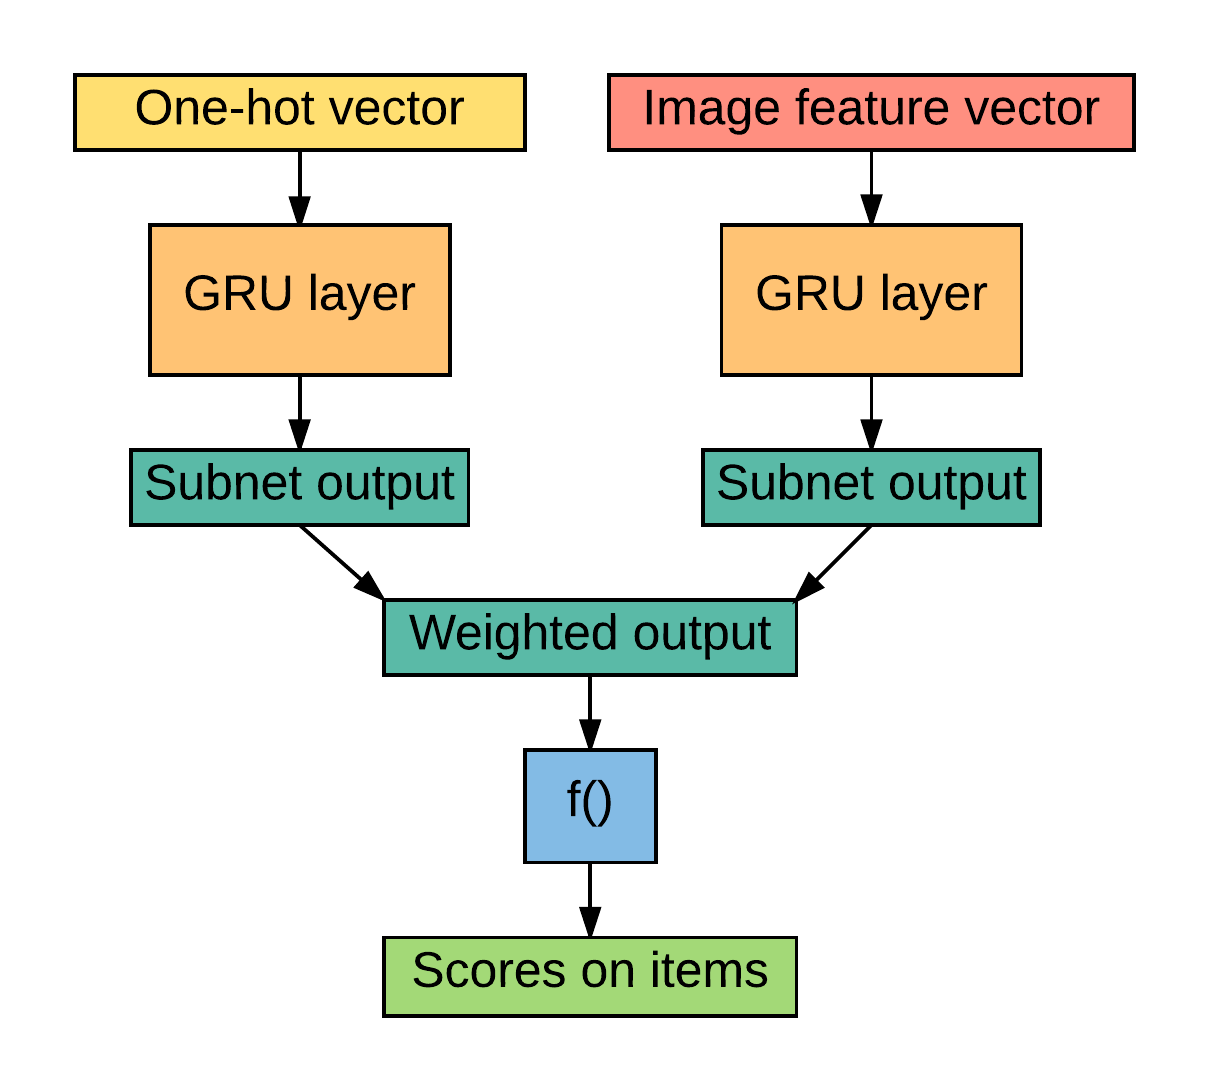
\includegraphics[width=1.0\textwidth]{fig/parallell-rnn.png}
	\caption{One of the proposed architectures from \cite{Hidasi:2016:PRN:2959100.2959167}. The image feature vector can be replaced with a text feature vector. f() is a nonlinearity applied to the output, in the paper they used tanh.}
	\label{fig:parallell-rnn}
\end{figure}

The two input vectors are fed into two separate GRU layers, and the outputs are combined by weighting each output. Lastly, the combined output is sent through an activation layer, giving scores for all possible items. The target label is the one-hot representation of the next event in the session. Two datasets were used, one with images of the items, and one with textual descriptions. The authors suggest different ways of training the models. Standard backpropagation can be suboptimal due to the parallelism of the architectures. The problem is that the different components can end up learning the same relations from the data \cite{Hidasi:2016:PRN:2959100.2959167}. As a baseline, the models are trained with simultaneous backpropagation on the whole model. To improve on this, they suggest alternating the training of the parallel components, i.e. the two GRU layers. Alternation can be done per mini-batch, per epoch, or across multiple epochs. Results are compared for the different architectures and the different training approaches.

Item-KNN was used as a baseline to compare the RNNs. Despite being simple, item-KNN is a strong basline in session-based recommendations, and often used in practice \cite{Hidasi:2016:PRN:2959100.2959167}. First the authors tested with 100 units in all GRU layers, the result was that all architectures outperformed the item-KNN baseline, except for the feature only model. The significantly best model was the one that is illustrated in Figure \ref{fig:parallell-rnn}. Afterwards, the best performing model, and the baseline models were tested again, but with larger GRU layers. The parallel model was tested with 500 units in each GRU layer, while the baseline models were tested with 1000 units in their GRU layer. Performance only slightly increased in the parallel model, but the feature only model was able to outperform the item-knn baseline. On the Recall@20 metric, the ID only (only had one-hot vector as input) model was able to perform as good as the parallel model. However, on the MRR@20 metric the parallel model was still significantly better. Also, comparison of the training approaches showed that the proposed ways of doing alternate training performed better than the simultaneous approach. When using large GRU layers, the best training approach was to interleave training of the GRU layers between each mini-batch. The results shows that even when increasing the capacity of the network has diminishing returns, the performance can still be improved by adding additional data sources \cite{Hidasi:2016:PRN:2959100.2959167}. And also that to include the additional data effectively, appropriate models with customized training should be used.

%touch shortly upon different methods that exists, but focus on 
%deep learning >> rnn

%what has been done in terms of using deep learning, rnn, +++ for recommender systems.

%---------------------------

%- how is rnn being used currently
%- how does rnn perform compared to other recsys models
%- touch extremely briefly upon what other recsys models are performing well now, and just link to explanations of them
%- talk about everything that other papers have achieved here?


\chapter{Core}


%explain the paper that i have tried to implement
%what did i want to achieve 
%core of what i implemented
\chapter{Experiments and results}

\section{Experiments}

\section{Results}

\section{Discussion}



%explain the experimental setting
%	explain the dataset that I have used
%		explain everything about the two datasets
%	talk about evaluation metrics 
%		how do they fit the recsys problem
%	which kind of testing
%	description of the experiment
	
%	results
	
%	discussion
\chapter{Conclusion and further work}
In this final chapter, we summarize our findings and look at interesting areas for further exploration.

\section{Conclusion}
In short, RNNs are very promising in the domain of session-based recommender systems. We have seen that they can compete with, and outperform, other state of the art models in this area. Deep learning also can be used to do most of the feature engineering for us. This has awakened the interests for RNNs as recommender systems in big companies such as Zalando, who are looking into the practical application of such models \cite{ZALANDO:understanding-consumer-histories}. 

We have seen that there are several ways to improve the basic RNN recommender. One of the most interesting improvements is to utilize more information than just the item clicks. Timestamps can be used in two different ways. Using the time between actions in a session can help the recommender understand which actions are relevant to each other. A long timespan between two actions might suggest that they are less relevant to each other, and that the RNN should forget much of what it know about the session. Time can also be used as an external context to the session. Time of day, day of week, month in the year, and whether it is a holiday, further helps the RNN to predict the most relevant items. Furthermore, additional information about both the action event and the corresponding item can be used. Often text or image is present and contains description of items. To use this efficiently, a good architecture must be chosen, and customized training also helps. We have looked at one such appropriate architecture, which used separate parallel GRU layers for the one-hot item encoding and the embedded description vector. Training the two GRU layers in an alternating fashion was shown to improve performance.

Different data augmentation techniques can also be helpful. One of the techniques was to pre-train the model on the full training set, and then fine-tune it on only the most recent examples. Intuitively this makes sense. We utilize the full training set, but focus the model on the most recent, up to date, examples. Older examples might contain trends that have later disappeared. 

A problem on news sites and other applications where items have a very short life cycle, is that the items in the training examples are not the same that will be recommended. The model can be retrained very frequently, but this requires a lot of fresh data, and is usually infeasible. The solution in these situations can be to embed items into a denser space where items with similar features are close in the embedded space. The model can then ''recommend'' an embedding, and the actual recommendations can be found by finding items that are close to the recommendation in the embedded space.

In applications where items have a longer life-cycle, such as in many e-commerce sites, the problem is sometimes the large number of items. The obvious solution is again to use embeddings. However, we have seen that this might reduce performance. 
 

\section{Further work}
There are two areas we want to look further into. First, improving the use of context information. In addition to using all the context and item information, we are interested in how we can use information from user actions that are not directly related to an item. E.g. search queries contain a lot of information about what the user is interested in, and should therefore be valuable information that can be utilized. 

Second, as the RNN processes a session, it learns an internal representation of the user-session. In the case where we have access to user identification, it could be possible to combine the user-session representations for a user to construct a dense representation of the user. We are interested in how this can be done, and if it can be used improve personalized recommendations.

%what is the future work
%have only looked at actions so fat
%we want to look at feeding in contextual data

%representation of the user

%- user representation with rnn (as the rnn works through a sequence, it stores a representation of user preferences, this could be used to represent the user. That is, the rnn creates a session representation and by combining these session representations for an individual user, it should be possible to represent the user.)
%- Use contextual information to improve the rnn recommender system

% Appendix
%%=========================================
\appendix
\chapter{List of Acronyms}

%\addcontentsline{toc}{section}{List of Acronyms}

% Keep these sorted alphabetically for extra readability

\begin{acronym}
    \acro{RNN}{Recurrent Neural Networks}
    \acro{LSTM}{Long Short Term Memory}
\end{acronym}
%\include{appendix-b}

\bibliographystyle{unsrt}
\bibliography{references}

\end{document}
% ==============================================
% ==============================================



% ==============================================
% =========== LATEX EXAMPLES ===================
% ==============================================

% =========== Code - listing ===================
\begin{lstlisting}
Put your code here.
\end{lstlisting}

\lstinputlisting[language=Python, firstline=37, lastline=45]{source_filename.py}

% =========== TODO =============================
\TODO{What to do}